\chapter{Results}

\section{Initial Results}
Initial data was collected from a non-real time version of the DGI code.
For each selected message arrival chance, as many as forty tests were run.
The collected results from the tests are divided into several target scenarios
as well as the protocol used.

The first minute of each test in the experimental test is discarded to remove
any transients in the test. The result is that while the tests were run for
ten minutes, the maximum result is 9 minutes of in-group time. These graphs
first appeared in \cite{CRITIS2012}.

\subsection{Sequenced Reliable Connection}

\subsubsection{Two Node Case}

\begin{figure}[!h]
\centering
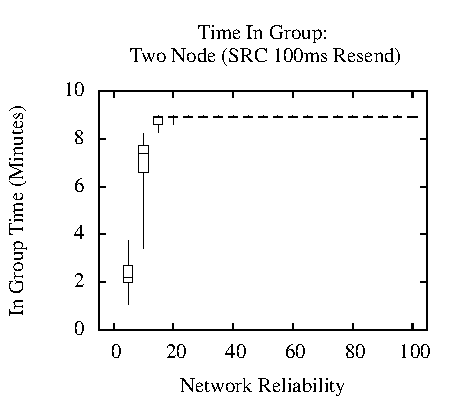
\includegraphics[width=\linewidth]{2NODE-SRC-100-GROUP.pdf}
\caption{Time in group over a 10 minute run for two node system with 100ms resend time}
\label{fig:IGT-SRC-2NODE-100}
\end{figure}

The 100ms resend SRC test with two nodes can be considered a sort of a control.
These tests, pictured in Figure \ref{fig:IGT-SRC-2NODE-100}, highlights the performance of the
SRC protocol, achieving the maximum in-group time of 9 minutes with only 15\%
of datagrams arriving at the receiver.

\begin{figure}[!h]
\centering
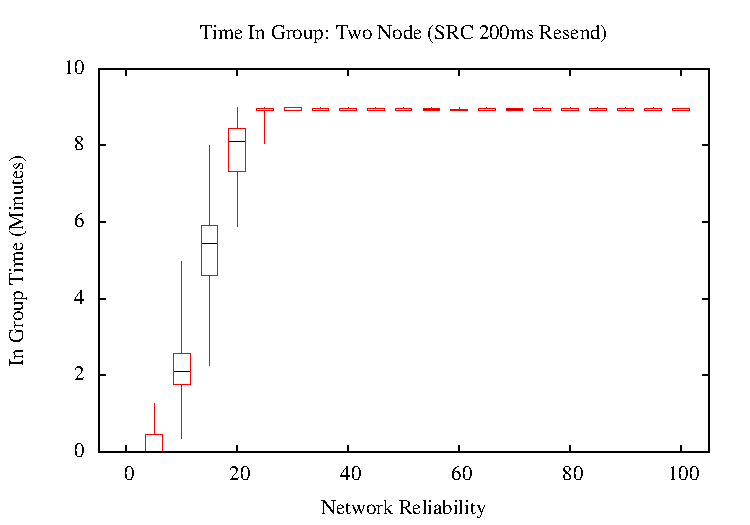
\includegraphics[width=\linewidth]{2NODE-SRC-200-GROUP.pdf}
\caption{Time in group over a 10 minute run for two node system with 200ms resend time}
\label{fig:IGT-SRC-2NODE-200}
\end{figure}

Figures \ref{fig:IGT-SRC-2NODE-200} demonstrates that as the
rate at which lost datagrams are resent is decreased to 200ms the
time in group falls off. This behavior is expected, since each exchange has a
time limit for each message to arrive and the number of attempts is reduced by
increasing the resend time.


\subsubsection{Transient Partition Case}

\begin{figure}[!h]
\centering
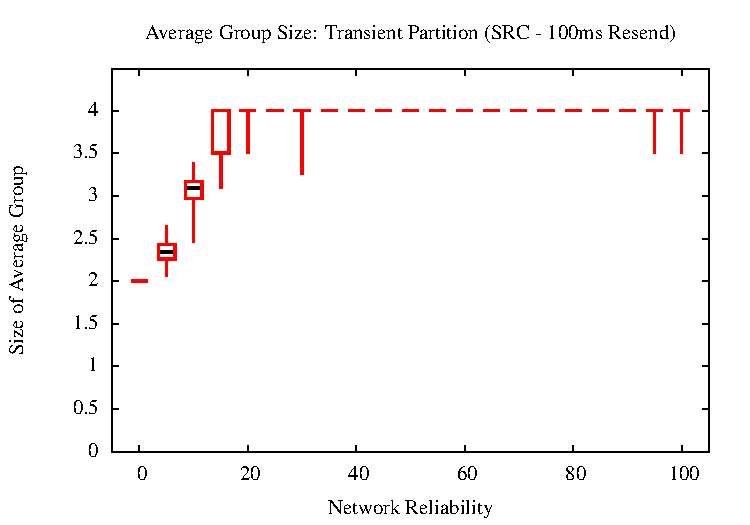
\includegraphics[width=\linewidth]{TRANS-SRC-100-SIZE.pdf}
\caption{Average size of formed groups for the transient partition case with 100ms resend time}
\label{fig:MGS-SRC-TRANS-100}
\end{figure}

\begin{figure}[!h]
\centering
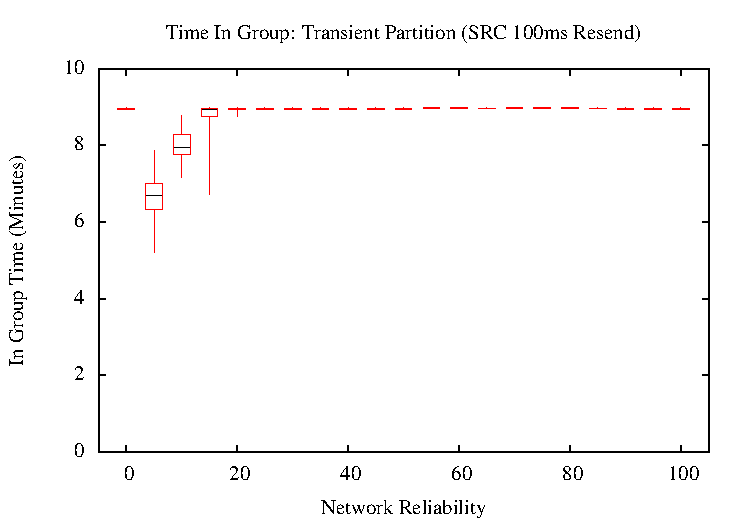
\includegraphics[width=\linewidth]{TRANS-SRC-100-GROUP.pdf}
\caption{Time in group over a 10 minute run for the transient partition case with 100ms resend time}
\label{fig:IGT-SRC-TRANS-100}
\end{figure}

The transient partition case shows a simple example where a network partition
separates two groups of DGI processes. In the simplest case where the opposite side of
the partition is unreachable, nodes will form a group with the other nodes on the
same side of the partition. In our tests, there are two nodes on each side of
the partition. In the experiment, the probability of a datagram crossing the
partition is increased as the experiment continues. The 100ms case is shown in
Figures \ref{fig:MGS-SRC-TRANS-100} and \ref{fig:IGT-SRC-TRANS-100}.

While messages cannot cross the partition, the DGIs stay in a group with the
nodes on the same side of the partition leading to an in group time of 9 minutes,
the maximum value. As packets begin to cross the partition (as the reliability
increases), DGI instances on either side begin to attempt to complete elections
with the nodes on the opposite partition and the time in group begins to fall.
However during this time, the mean group size continues to increase, meaning
while the elections are decreasing the amount of time that the module spends in
state where it can actively do work, it typically does not fall into a state
where it is in a group by itself, which means that most of the lost in-group
time comes from elections.

\begin{figure}[!h]
\centering
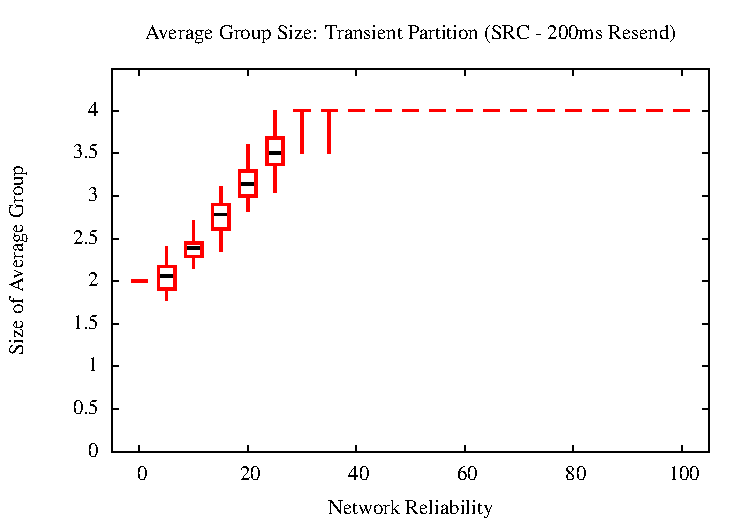
\includegraphics[width=\linewidth]{TRANS-SRC-200-SIZE.pdf}
\caption{Average size of formed groups for the transient partition case with 200ms resend time}
\label{fig:MGS-SRC-TRANS-200}
\end{figure}

\begin{figure}[!h]
\centering
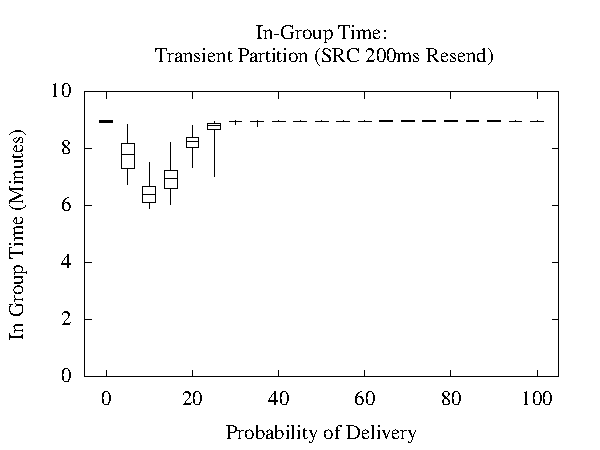
\includegraphics[width=\linewidth]{TRANS-SRC-200-GROUP.pdf}
\caption{Time in group over a 10 minute run for the transient partition case with 200ms resend time}
\label{fig:IGT-SRC-TRANS-200}
\end{figure}

The 200ms case, shown in Figures \ref{fig:MGS-SRC-TRANS-200} and \ref{fig:IGT-SRC-TRANS-200} displays similar behavior, with a wider valley due to the
limited number of datagrams. It is also worth noting the that the mean group
size dips below 2 in the figure, possibly because the longer resend times allow
for more race conditions between potential leaders. Discussion of these race
conditions is shown in discussed during the SUC charts since it is more prevalent
in those experiments.

\subsection{Sequenced Unreliable Connection}

\subsubsection{Two Node Case}

The SUC protocol's experimental tests show an immediate problem: although there
is a general trend of growth in the amount of time in group and group size
charts, shown in Figure \ref{fig:IGT-SUC-2NODE-100}
there is a high amount of variance for any particular trial.

\begin{figure}[!h]
\centering
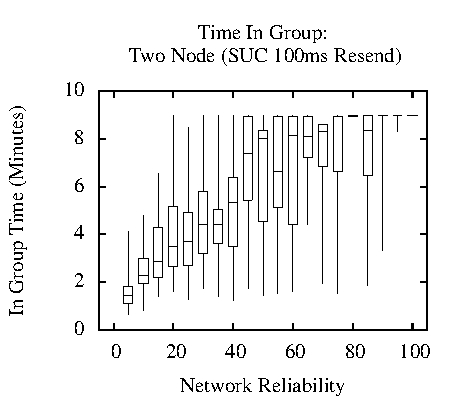
\includegraphics[width=\linewidth]{2NODE-SUC-100-GROUP.pdf}
\caption{Time in group over a 10 minute run for two node system with 100ms resend time}
\label{fig:IGT-SUC-2NODE-100}
\end{figure}

\begin{figure}[!h]
\centering
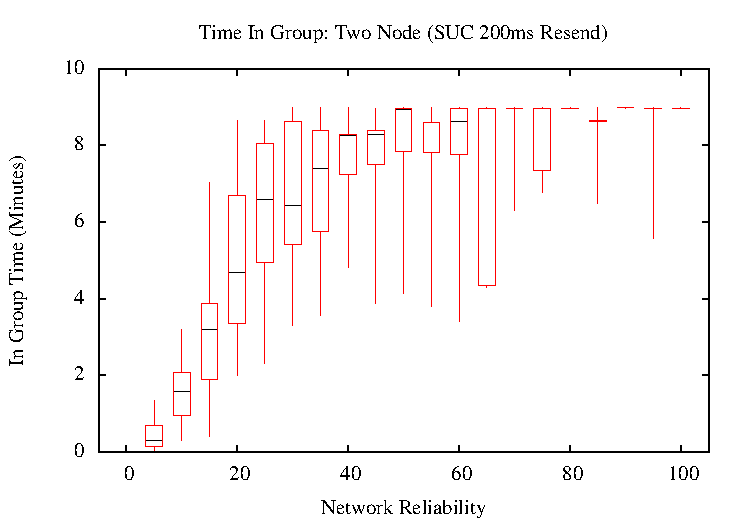
\includegraphics[width=\linewidth]{2NODE-SUC-200-GROUP.pdf}
\caption{Time in group over a 10 minute run for two node system with 200ms resend time}
\label{fig:IGT-SUC-2NODE-200}
\end{figure}

In the 200ms resend case, show in Figure \ref{fig:IGT-SUC-2NODE-200}, it can be
observed that there is a more growth rate in the in-group time as a the
reliability increases. In fact, averaging across all the collected data points
from the experiment, the average in-group time is higher for the 200ms case
than it is for the 100ms case ( 6.86 vs 6.09 ). However, due to the large amount
of variance in the collected in-group time, it is not possible to state with
confidence that the there is a significant difference between the two cases.

\section{Markov Models}

Due to the high amount of variance in the collected data, and the resulting
difficulty making any sort of prediction about other systems from the data, a
more formal approach was tried.

\subsection{Initial Model Calibration}
The presented methodology of constructing the model was initially calibrated against the
original two-node case, using a non-real-time version of the DGI codebase. The resulting
Markov chain was processed using SharpE \cite{SHARPE}\cite{SHARPE2} made by Dr. Kishor
Trivedi's group at Duke University, a popular tool for reliability analysis. SharpE measured the reward collected in 600 seconds,
minus the reward that was collected in the first 60 seconds (to emulate that the first
60 seconds were discarded in the experimental runs.) The SharpE results are plotted along
with the experimental results in Figures \ref{fig:COMPARE-SUC-2NODE-100} and \ref{fig:COMPARE-SUC-2NODE-200}.

\begin{figure}[!h]
\centering
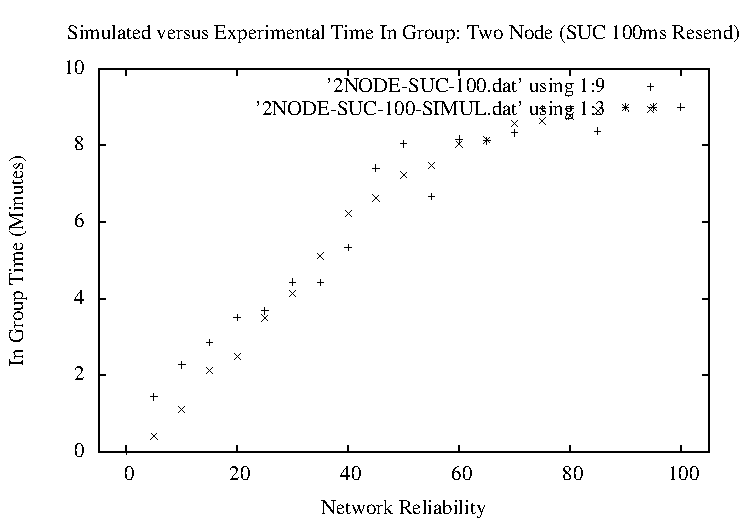
\includegraphics[width=1.0\linewidth]{2NODE-SUC-100-COMPARE.pdf}
\caption{Comparison of in-group time as collected from the experimental platform and the simulator (1 tick offset between processes).}
\label{fig:COMPARE-SUC-2NODE-100}
\end{figure}


\begin{figure}[!h]
\centering
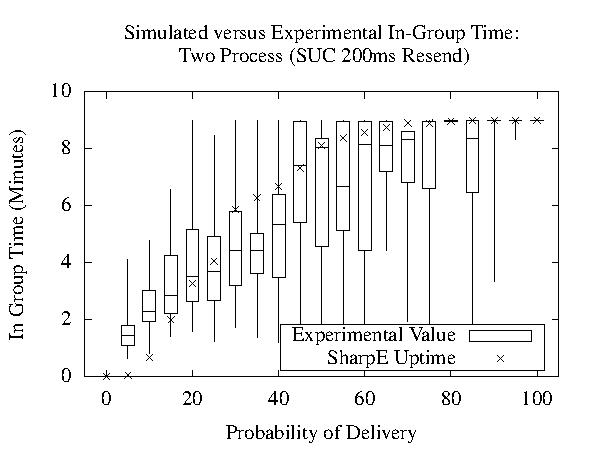
\includegraphics[width=1.0\linewidth]{2NODE-SUC-200-COMPARE.pdf}

\caption{Comparison of in-group time as collected from the experimental platform and the simulator (2 tick offset between processes).}
\label{fig:COMPARE-SUC-2NODE-200}
\end{figure}

The race condition between processes during an election is a consideration in the original
leader election algorithm, and is an additional factor here. The simulator provided a parameter
to allow the operator to select how closely synchronized the peers were (the time difference
between when each of them would search for leaders.) The exchange of messages, particularly
during an election had a tendency to synchronize nodes during elections, and so the nodes could
synchronize even if they did not initially begin in a synchronized state. As a result, the
simulation results aligned best for the 100ms resend case with 1 ticks (Approximately 100ms
difference in synchronization between processes) and 2 ticks (Approximately 400ms) in the 200ms
resend case.

Models fit to the non-real-time code in groups larger than 2 processes did not fit well.
This is presumed to be a combination of several factors. The suspected major source of fault
included the structure of the chain, which naturally assumes that all processes enter the
election state a roughly the same time, which is not typically true for any number of processes
greater than 2. Additionally, the simulator could only assume that the synchronization between
processes was mostly fixed, which was not the case in the larger configurations, since the
coincidental synchronization that occurred in the two node case was suppressed by the increased
number of peers. Furthermore, an issue with SharpE was discovered that prevented the
particular structure of the chains produced from being handled correctly. To circumvent that,
issue, SharpE was replaced by a random-walker which generates exponentially distributed numbers
and follows the paths of the chain, across several hundred trials, in order to collect time in group data for
models which SharpE cannot process.

The structure of the Markov Chain, which assumed that processes enter the election state
mostly simultaneously was an appropriate assumption for the real-time system, since the
round-robin scheduler synchronizes when processes run their group management modules. The
simulator was set to assume that the synchronization between processes was very tight, and
new experimental data was collected for the 4 node, transient partition case. The collected
data is overlaid with the results from the random walker in Figures \ref{fig:COMPARE-SUC-TRANS-RT-128} and \ref{fig:COMPARE-SUC-TRANS-RT-64}.

\begin{figure}[!h]
\centering
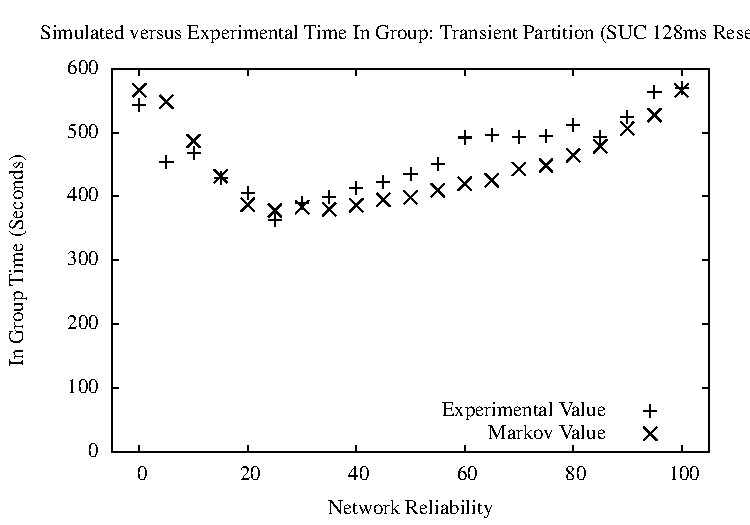
\includegraphics[width=1.0\linewidth]{TRANS-RT-SUC-128-COMPARE.pdf}
\caption{Comparison of in-group time as collected from the experimental platform and the time in group from the equivalent Markov chain (128ms between resends).}
\label{fig:COMPARE-SUC-TRANS-RT-128}
\end{figure}

\begin{figure}[!h]
\centering
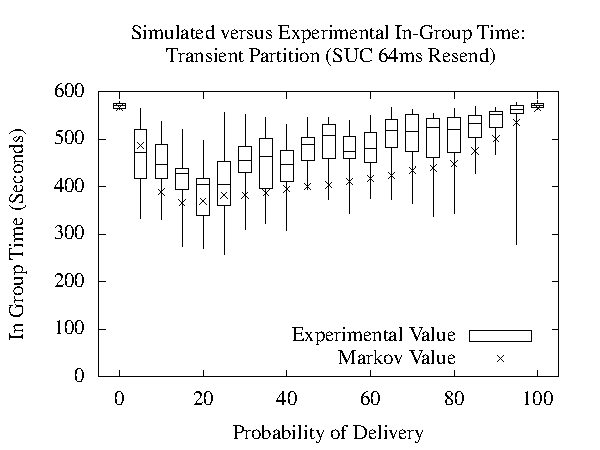
\includegraphics[width=1.0\linewidth]{TRANS-RT-SUC-64-COMPARE.pdf}

\caption{Comparison of in-group time as collected from the experimental platform and the time in group from the equivalent Markov chain (64ms between resends).}
\label{fig:COMPARE-SUC-TRANS-RT-64}
\end{figure}

As a measure of the strength of the model, the correlation between the predicted value was compared.
The average error was also computed for each of the samples taken. This information is presented in
Table \ref{tab:STAT-DATA}.

\begin{table}
% increase table row spacing, adjust to taste
\caption{Error and correlation of experimental data and Markov chain predictions}
\label{tab:STAT-DATA}
\centering
% Some packages, such as MDW tools, offer better commands for making tables
% than the plain LaTeX2e tabular which is used here.
\begin{tabular}{|c||c|c|c|}
\hline
Resend & Correlation & Error \\ \hline
128 & 0.7656 & 11.61\% \\ \hline
64 & 0.8604 & 11.70\% \\ \hline
\end{tabular}
\end{table}


